% =================================================================
% Supplementary material. Compiled after main.tex (labels are read from
% main.aux through xr-hyper) and appended to main.pdf by qa/build_pdf.sh.
% Build: xelatex main (x3, bibtex) && xelatex supplement && xelatex supplement
% =================================================================
\documentclass[fontset=none,10pt,a4paper]{ctexart}
\usepackage{iftex}
\ifXeTeX\else
  \PackageError{paper-template}{XeLaTeX is required}{Run xelatex.}
\fi
\usepackage{fontspec}
\IfFontExistsTF{Times New Roman}{
  \setmainfont{Times New Roman}
}{
  \setmainfont{Liberation Serif}
}
\IfFontExistsTF{SimSun}{
  \IfFontExistsTF{SimHei}{
    \setCJKmainfont[BoldFont=SimHei]{SimSun}
  }{
    \setCJKmainfont[AutoFakeBold=2.5]{SimSun}
  }
}{
  \IfFontExistsTF{Songti SC}{
    \setCJKmainfont{Songti SC}
  }{
    \IfFontExistsTF{STSong}{
      \setCJKmainfont{STSong}
    }{
      \setCJKmainfont{Noto Serif CJK SC}
    }
  }
}
\IfFontExistsTF{SimHei}{
  \setCJKsansfont{SimHei}
}{
  \IfFontExistsTF{Heiti SC}{\setCJKsansfont{Heiti SC}}{\setCJKsansfont{Noto Sans CJK SC}}
}
\usepackage{graphicx}
\usepackage{amsmath,amsthm}
% OpenType math font: every math glyph carries a Unicode mapping in the text layer.
\usepackage{unicode-math}
\IfFontExistsTF{Latin Modern Math}{
  \setmathfont{Latin Modern Math}
}{
  \setmathfont{Cambria Math}
}
% Estimator hats drawn as vector polylines so that accents do not overlap letters in the text layer.
\usepackage{pict2e}
\DeclareRobustCommand{\hatmark}{{\setlength{\unitlength}{0.1em}\linethickness{0.045em}%
  \begin{picture}(5,1.7)\polyline(0.2,0)(2.5,1.5)(4.8,0)\end{picture}}}
\AtBeginDocument{%
  \renewcommand{\widehat}[1]{\overset{\hatmark}{#1}}%
  \renewcommand{\hat}[1]{\overset{\hatmark}{#1}}}
\usepackage[a4paper, margin=0.8in]{geometry}
\usepackage[round,authoryear]{natbib}
\usepackage{booktabs}
\usepackage{microtype}
\usepackage{xcolor}
\usepackage{enumitem}
\usepackage{array}
\usepackage{xurl}
\usepackage{xr-hyper}
\usepackage[hidelinks,unicode=true]{hyperref}
\usepackage{refcount}
\urlstyle{same}
\usepackage{caption}
\usepackage{subcaption}
\usepackage{placeins}
\captionsetup{
  font=small,
  labelfont=normalfont,
  textfont=normalfont,
  labelsep=space,
  justification=justified,
  singlelinecheck=true,
  skip=6pt
}
\setlength{\textfloatsep}{12pt plus 2pt minus 2pt}
\setlength{\floatsep}{10pt plus 2pt minus 2pt}
\setlength{\intextsep}{10pt plus 2pt minus 2pt}
\setcounter{topnumber}{5}
\setcounter{bottomnumber}{3}
\setcounter{totalnumber}{8}
\renewcommand{\topfraction}{0.90}
\renewcommand{\bottomfraction}{0.80}
\renewcommand{\textfraction}{0.07}
\renewcommand{\floatpagefraction}{0.70}
\pagestyle{plain}
\setlist{nosep,leftmargin=2em}

\newtheoremstyle{zhplain}{0.6em}{0.6em}{\normalfont}{}{\sffamily}{}{0.8em}{}
\theoremstyle{zhplain}
\newtheorem{sproposition}{补充命题}
\renewcommand{\thesproposition}{S\arabic{sproposition}}
\renewcommand{\proofname}{证明}

\newcommand{\Rbar}{\overline{R}}
\newcommand{\mx}{m_{\times}}
\newcommand{\NB}{\operatorname{NB}}
\newcommand{\Var}{\operatorname{Var}}
\newcommand{\E}{\operatorname{E}}
\newcommand{\Cov}{\operatorname{Cov}}
\newcommand{\CV}{\operatorname{CV}}
\newcommand{\Bin}{\operatorname{Bin}}
\newif\ifblind
\blindfalse
\externaldocument{build/main}
\renewcommand{\thesection}{S\arabic{section}}
\renewcommand{\theequation}{S\arabic{equation}}
\renewcommand{\thetable}{S\arabic{table}}
\renewcommand{\thefigure}{S\arabic{figure}}

\title{\textbf{补充材料：环境方差与报告异质性下再生数估计的不可约误差与监测设计}}
\ifblind
  \author{匿名作者}
\else
  \author{王驰\\[2pt]{\small 西安科技大学}}
\fi
\date{}

\begin{document}
\setcounter{page}{\numexpr\getpagerefnumber{LastPage}+1\relax}
\maketitle
\thispagestyle{plain}
\normalfont\mdseries

\section{命题的证明}
\label{app:proofs}

本节给出正文第~\ref{sec:results}~节各命题、推论与注的证明和推导，以及第~\ref{sec:meth-renewal}~节的方差推导。正文的命题、推论、注与式号沿用正文编号，本节新增的式号带前缀 S。

负二项分布 $\NB(r,p)$ 的均值与方差为 $r(1-p)/p$ 与 $r(1-p)/p^2$。取 $r=k$、$p=k/(k+R)$ 即得式~\eqref{eq:offspring}；求和与二项稀疏的结论见第~\ref{sec:meth-model}~节式~\eqref{eq:thinning}，代入 $p=k/(k+R_t)$ 时 $q=(k+\rho R_t)/(k+R_t)$。式~\eqref{eq:relvar} 由式~\eqref{eq:report-dist} 的均值与方差直接相除得到。

\subsection{\texorpdfstring{命题~\ref{prop:current} 的证明}{命题 1 的证明}}

记 $c$ 为 $C_t$ 的观测值，$\theta=\rho R_t$。由式~\eqref{eq:report-dist}，对数似然为 $\ell(R_t)=\text{const}+nk\log[k/(k+\theta)]+c\log[\theta/(k+\theta)]$。对 $R_t$ 求导并整理，得分函数为：
\begin{equation}
  \dot\ell(R_t)=\frac{c}{R_t}-\frac{(c+nk)\rho}{k+\rho R_t}
  =\mathcal I(R_t)\,(\widehat R_t-R_t),\qquad
  \mathcal I(R_t)=\frac{k\rho n}{R_t(k+\rho R_t)}=\frac{n}{R_t/\rho+{R_t}^2/k}.
  \label{eq:score}
\end{equation}

(i) 当 $c>0$ 时，由式~\eqref{eq:score}，得分函数在 $R_t<\widehat R_t$ 时为正，在 $R_t>\widehat R_t$ 时为负，似然在 $\widehat R_t$ 处取唯一最大值。当 $c=0$ 时，$\dot\ell(R_t)=-nk\rho/(k+\rho R_t)<0$，似然在 $(0,\infty)$ 上严格递减，最大值在边界 $R_t=0$，与 $\widehat R_t=0$ 一致。

(ii) 由式~\eqref{eq:report-dist}，$\E\widehat R_t=\rho nR_t/(\rho n)=R_t$，且
\begin{equation}
  \Var(\widehat R_t)=\frac{\rho nR_t+\rho^2nR_t^2/k}{(\rho n)^2}=\frac{R_t}{\rho n}+\frac{R_t^2}{kn}=\frac{R_t(k+\rho R_t)}{k\rho n}.
\end{equation}

(iii) Fisher 信息为得分函数的方差。由式~\eqref{eq:score} 与 (ii) 得
\begin{equation}
  \mathcal I(R_t)=\frac{(k\rho n)^2}{[R_t(k+\rho R_t)]^2}\Var(\widehat R_t)=\frac{k\rho n}{R_t(k+\rho R_t)}=\frac{n}{R_t/\rho+{R_t}^2/k}.
\end{equation}
因此 $\Var(\widehat R_t)=1/\mathcal I(R_t)$。得分函数是 $\widehat R_t-R_t$ 的倍数，这正是 Cramér--Rao 不等式取等号的充要条件\citep{casella2002statistical}，对每个有限 $n$ 都成立。

(iv) 式~\eqref{eq:report-dist} 的概率函数可写为只依赖 $c$ 的因子乘以 $\exp[\upsilon c-\mathcal A(\upsilon)]$，其中自然参数 $\upsilon=\log[\rho R_t/(k+\rho R_t)]$，$\mathcal A$ 为对数配分函数。$k$ 已知时它属于单参数指数族；$R_t$ 取遍 $(0,\infty)$ 时，$\upsilon$ 取遍 $(-\infty,0)$，含开区间，所以 $C_t$ 是完备充分统计量。$\widehat R_t$ 是 $C_t$ 的函数且无偏，由 Lehmann--Scheffé 定理，它是一致最小方差无偏估计\citep{casella2002statistical}。\qed

\subsection{\texorpdfstring{命题~\ref{prop:average} 的证明}{命题 2 的证明}}

由 H4，给定 $n$ 时 $R_t$ 的均值与方差为 $\Rbar$ 与 $v_R$。由命题~\ref{prop:current}(ii)，$\E(\widehat R_t\mid n,R_t)=R_t$，所以 $\E(\widehat R_t\mid n)=\Rbar$。由全方差公式
\begin{equation}
  \Var(\widehat R_t\mid n)=\E\{R_t/(\rho n)+R_t^2/(kn)\mid n\}+\Var(R_t\mid n)
  =\frac{\Rbar}{\rho n}+\frac{\Rbar^2+v_R}{kn}+v_R.
\end{equation}
以 $m=\rho n$ 代入，前两项之和为 $A/m$，得式~\eqref{eq:var-average}。

(i) $A/m\to0$。(ii) 规模项份额为 $(A/m)/(v_R+A/m)=1/(1+mv_R/A)=1/(1+m/\mx)$。(iii) 翻倍降幅为 $[V(m)-V(2m)]/V(m)=[A/(2m)]/(v_R+A/m)=1/[2(1+m/\mx)]$。(iv) $V'(m)=-A/m^2<0$，$V''(m)=2A/m^3>0$；弹性为 $mV'(m)/V(m)=-(A/m)/(v_R+A/m)=-\mx/(m+\mx)$，在 $m=\mx$ 处为 $-1/2$。

(v) 设 $\tilde\theta$ 只依赖本期报告数且 $\E(\tilde\theta\mid R_t)=R_t$。给定 $R_t$，它是 $R_t$ 的无偏估计，由 Cramér--Rao 不等式，$\Var(\tilde\theta\mid R_t)\geq1/\mathcal I(R_t)$。代入式~\eqref{eq:unbiased-bound} 的分解，$\E(\tilde\theta-\Rbar)^2\geq v_R+\E[1/\mathcal I(R_t)]=V(m)$，$\widehat R_t$ 取等号。一步预测时，$y=C_{t+1}/m$，$\hat y$ 由 $\mathcal F_t$ 决定。由 H4，$R_{t+1}$ 与 $\mathcal F_t$ 独立，$C_{t+1}$ 在 $\mathcal F_t$ 下的条件分布与 $\mathcal F_t$ 无关，于是 $\E[(\hat y-y)^2\mid\mathcal F_t]=(\hat y-\E y)^2+\Var(y)\geq\Var(y)=V(m)$，$\hat y=\Rbar$ 取等号。\qed

式~\eqref{eq:pooling} 的推导如下。$J$ 个环境项方差同为 $v_R$、两两相关系数平均为 $\bar c$ 时，其等权平均的方差为 $J^{-2}[Jv_R+J(J-1)\bar cv_R]=v_R[\bar c+(1-\bar c)/J]$。

\subsection{\texorpdfstring{注~\ref{rem:reporting} 的推导}{注 1 的推导}}

把式~\eqref{eq:var-average} 写成 $n$ 与 $\rho$ 的函数
\begin{equation}
  V(n,\rho)=v_R+\frac{\Rbar}{\rho n}+\frac{\Rbar^2+v_R}{kn}.
\end{equation}
令 $\rho\to1$，第二项趋于 $\Rbar/n>0$，第三项与 $\rho$ 无关且为正，故极限严格大于 $v_R$；令 $n\to\infty$，后两项都趋于零。两个方向的边际效应为
\begin{equation}
  -\frac{\partial V}{\partial\log n}=\frac{\Rbar}{\rho n}+\frac{\Rbar^2+v_R}{kn}=\frac{A}{m},\qquad
  -\frac{\partial V}{\partial\log\rho}=\frac{\Rbar}{\rho n}=\frac{\Rbar}{m}.
\end{equation}
二者之比为 $A/\Rbar=1+\rho(\Rbar^2+v_R)/(k\Rbar)$。

\subsection{\texorpdfstring{命题~\ref{prop:allocation} 的证明}{命题 3 的证明}}

(i) 设各期上一代人数均为 $n$，给定 $(R_1,\dots,R_T)$ 时各期报告数相互独立。记 $\bar R_T=T^{-1}\sum_tR_t$。由全方差公式
\begin{equation}
  \frac{1}{T^2}\Var({\textstyle\sum_t}\widehat R_t)=\Var(\bar R_T)+\frac1{T^2}\sum_t\E\{R_t/(\rho n)+R_t^2/(kn)\}
  =\Var(\bar R_T)+\frac{A}{Tm}.
\end{equation}
右端第二项等于 $A/B$，只依赖 $R_t$ 的边际分布，与相关结构无关。$R_t$ 独立时 $\Var(\bar R_T)=v_R/T$，得式~\eqref{eq:alloc-indep}。

一阶自回归情形下，$\Cov(R_s,R_t)=v_R\phi^{|s-t|}$，于是
\begin{equation}
  T^2\Var(\bar R_T)=v_R\,T+2v_R\sum_{h=1}^{T-1}(T-h)\phi^h,\qquad
  \sum_{h=1}^{T-1}(T-h)\phi^h=\frac{\phi[T(1-\phi)-(1-\phi^T)]}{(1-\phi)^2}.
\end{equation}
后一个等式可对 $T$ 归纳验证。代入整理即得式~\eqref{eq:ar-sum}。

单调性。记 $M_T=T^2\Var(\bar R_T)$，$\Delta_j=v_R(1+2\sum_{h=1}^{j}\phi^h)$，则 $M_{T+1}=M_T+\Delta_T$，$M_T=\sum_{j=0}^{T-1}\Delta_j$。$\Var(\bar R_{T+1})<\Var(\bar R_T)$ 等价于 $T^2\Delta_T<(2T+1)M_T$。数列 $\Delta_j$ 的增量 $2v_R\phi^{j+1}$ 递减，所以它是凹数列，满足 $\Delta_j\geq[(T-j)\Delta_0+j\Delta_T]/T$。对 $j=0,\dots,T-1$ 求和，得 $M_T\geq[(T+1)\Delta_0+(T-1)\Delta_T]/2$。记 $d=\Delta_T-\Delta_0$，代入 $\Delta_0=v_R$，有
\begin{equation}
  (2T+1)M_T-T^2\Delta_T\geq(T+1)(Tv_R-d/2).
\end{equation}
由于 $d=2v_R\sum_{h=1}^{T}\phi^h<2Tv_R$，右端为正。$\phi=0$ 时即独立情形，单调性显然成立。

(ii) 由式~\eqref{eq:alloc-indep}，以 $T=\mathcal B/(c_0+c_1m)$、$B=Tm$ 代入，得
\begin{equation}
  f(m)=\frac{(c_0+c_1m)(v_R+A/m)}{\mathcal B}=\frac{c_0v_R+c_1A+c_1v_Rm+c_0A/m}{\mathcal B}.
\end{equation}
$f'(m)=(c_1v_R-c_0A/m^2)/\mathcal B$，$f''(m)=2c_0A/(m^3\mathcal B)>0$。$c_0>0$ 时 $f$ 在 $(0,\infty)$ 上严格凸，唯一驻点为 $m^{*2}=c_0A/(c_1v_R)=(c_0/c_1)\mx$。代回得 $f(m^*)=[c_0v_R+c_1A+2\sqrt{c_0c_1v_RA}]/\mathcal B$，即式~\eqref{eq:optimal-m}。

约束 $T\geq1$ 等价于 $m\leq(\mathcal B-c_0)/c_1$。若 $m^*$ 超出可行范围，$f$ 在可行区间上递减，最优解取右端点，即 $T=1$。若 $c_0=0$，$f(m)=c_1(v_Rm+A)/\mathcal B$ 严格递增，下确界在 $m\to0$ 处取得。

整数解。$m=(\mathcal B/T-c_0)/c_1$ 关于 $T$ 单调，而 $f$ 关于 $m$ 单峰，所以 $f$ 作为 $T$ 的函数也单峰，整数最优解是连续最优期数两侧的两个整数之一，正文的取整例子即按此比较。环境服从一阶自回归时的精确结果见命题~\ref{prop:ar-design}。\qed

\subsection{增长检验的证明}
\label{sec:s-test}

正文第~\ref{sec:res-test}~节的增长检验以 $C_t\geq c_\alpha$ 为拒绝域，下面给出其三条性质的证明。

取 $R>R'$。由式~\eqref{eq:report-dist}，两者的似然比为
\begin{equation}
  \frac{f(c;R)}{f(c;R')}=\frac{(k+\rho R')^{nk}\,[R(k+\rho R')]^{c}}{(k+\rho R)^{nk}\,[R'(k+\rho R)]^{c}}.
\end{equation}
由于 $R/(k+\rho R)$ 关于 $R$ 严格递增，$R(k+\rho R')/[R'(k+\rho R)]>1$，似然比关于 $c$ 严格递增，分布族具有单调似然比。

(a) 水平。对单调似然比族，形如 $\{C_t\geq c\}$ 的检验的功效函数关于 $R_t$ 非降\citep{lehmann2005testing}，所以在 $R_t\leq1$ 上的最大拒绝概率在 $R_t=1$ 处取得，等于 $\alpha^*=P_{R_t=1}(C_t\geq c_\alpha)\leq\alpha$。

(b) 一致最优。由 Karlin--Rubin 定理\citep{karlin1956theory}，对任意水平，形如“$C_t>c$ 时拒绝，$C_t=c$ 时以概率 $\gamma$ 拒绝”的检验在该水平下一致最优。非随机检验 $\{C_t\geq c_\alpha\}$ 是 $c=c_\alpha-1$、$\gamma=1$ 的特例，所以在水平 $\alpha^*$ 下一致最优；适当选取 $\gamma$ 可以使水平恰为 $\alpha$。

(c) 功效。$R_t=1+\delta$ 时，$C_t\sim\NB(nk,k/[k+\rho(1+\delta)])$，拒绝概率为 $1-F_{\NB}(c_\alpha-1)$，即式~\eqref{eq:power}。\qed

\subsection{\texorpdfstring{命题~\ref{prop:report-noise} 与推论~\ref{cor:switch} 的证明}{命题 4 与推论 1 的证明}}

(i) 给定 $(n,R_t,p_t)$，由式~\eqref{eq:report-dist}，$\E(C_t\mid\cdot)=p_tnR_t$，$\Var(C_t\mid\cdot)=p_tnR_t+p_t^2nR_t^2/k$。对 $p_t$ 用全方差公式，并代入 $\E p_t=\rho$、$\E p_t^2=\rho^2+\sigma^2$，得：
\begin{equation}
  \Var(C_t\mid n,R_t)=\rho nR_t+\frac{(\rho^2+\sigma^2)nR_t^2}{k}+\sigma^2n^2R_t^2 .
\end{equation}

(ii) $\E(C_t\mid n,R_t)=\rho nR_t$，所以 $\E\widehat R_t=\Rbar$。再对 $R_t$ 用全方差公式，$\Var(\E(\widehat R_t\mid R_t))=v_R$，条件方差的期望为 $(\rho n)^{-2}\E[\Var(C_t\mid n,R_t)]$。代入 $\E R_t^2=\Rbar^2+v_R$ 与 $m=\rho n$，得：
\begin{equation}
  V_H(m)=v_R+\frac{\sigma^2}{\rho^2}(\Rbar^2+v_R)+\frac{\Rbar}{m}+\frac{(\rho^2+\sigma^2)(\Rbar^2+v_R)}{\rho km},
\end{equation}
整理即为式~\eqref{eq:r3-vH}。第二项不含 $n$。

(iii) 记 $\theta_t=p_tR_t=\rho R_tu_t$。给定 $\theta_t$ 时 $C_t$ 的分布 $\NB(nk,k/(k+\theta_t))$ 与 $R_t$ 无关，$R_t\to\theta_t\to C_t$ 构成马尔可夫链。由 Fisher 信息的数据处理不等式\citep{zamir1998proof}：
\begin{equation}
  \mathcal I_{C_t}(R_t)\ \leq\ \mathcal I_{\theta_t}(R_t)=\frac{\mathcal J_u}{R_t^2},
\end{equation}
其中等号右端是尺度族 $\theta_t/\rho=R_tu_t$ 关于尺度参数的 Fisher 信息，其密度为 $f_u(y/R)/R$，对 $R$ 求导后在 $u=y/R$ 处得分函数为 $-[1+uf_u'(u)/f_u(u)]/R$。对条件无偏估计量用给定 $R_t$ 的 Cramér--Rao 不等式，$\Var(\tilde\theta\mid R_t)\geq R_t^2/\mathcal J_u$；再按式~\eqref{eq:unbiased-bound} 的方式对 $R_t$ 取期望，即得式~\eqref{eq:r3-lb} 的第一个不等式。

记尺度族的得分函数为 $s_u(u)=-[1+uf_u'(u)/f_u(u)]$（取 $R=1$）。$\E u_t=1$ 对尺度参数求导得 $\E[s_u(u_t)\,u_t]=1$，又 $\E s_u(u_t)=0$，故 $\Cov(s_u(u_t),u_t)=1$。由 Cauchy--Schwarz 不等式，$1\leq\mathcal J_u\Var(u_t)=\mathcal J_u\tau^2$，即 $\mathcal J_u\geq1/\tau^2$。等号成立当且仅当 $s_u(u)=b_u(u-1)$，即 $f_u'(u)/f_u(u)=(b_u-1)/u-b_u$，解得 $f_u(u)\propto u^{b_u-1}e^{-b_uu}$，为形状与速率同为 $b_u=1/\tau^2$ 的 Gamma 分布。此时下界为 $v_R+\tau^2(\Rbar^2+v_R)=v_R+v_H$，对每个 $m$ 成立；$\widehat R_t$ 的均方误差为 $v_R+v_H+A_H/m$，$m\to\infty$ 时趋于下界，下确界因此为 $v_R+v_H$。对数正态 $u_t=\exp(sZ-s^2/2)$ 时，$s_u(u)=(\ln u+s^2/2)/s^2$，$\mathcal J_u=1/s^2$，而 $\tau^2=e^{s^2}-1$，故 $(\Rbar^2+v_R)/\mathcal J_u=v_H\log(1+\tau^2)/\tau^2$。


(iv) 给定 $(R_t,p_t)$，$\E(C_t\mid\cdot)=p_tnR_t$，$\tilde R_t=C_t/(p_tn)$ 的条件方差为 $R_t/(p_tn)+R_t^2/(kn)$。条件均值 $R_t$ 的方差为 $v_R$；对 $(R_t,p_t)$ 取期望并利用二者独立，即得式~\eqref{eq:r3-obs}。$\E(1/p_t)$ 有限保证式中第二项有限。二项型波动下 $\E(1/p_t)=B(\rho\nu-1,(1-\rho)\nu)/B(\rho\nu,(1-\rho)\nu)=(\nu-1)/(\rho\nu-1)$，要求 $\rho\nu>1$；$\rho\nu\leq1$ 时 Beta 密度在 0 附近的质量使 $\E(1/p_t)$ 发散。$\rho=0.25$、$\nu=100$ 时 $\E(1/p_t)=4.125$。制度型波动取 $u_t$ 服从形状与速率同为 $1/\tau^2$ 的 Gamma 分布时，$\E(1/u_t)=1/(1-\tau^2)$，要求 $\tau<1$。

(v) 由 (ii)，$v_R+v_H=(1+\tau^2)(\Rbar^2+v_R)-\Rbar^2=U-\Rbar^2$，$A_H=\Rbar+\rho U/k$，$\E\widehat R_t=\Rbar$ 不含 $v_R$ 与 $\tau^2$。$(v_R,\tau^2)$ 沿 $U$ 的等值线变化时，报告数的均值与方差都不变。

(vi) 无计数噪声时 $C_{j,t}=\rho_ju_{j,t}I_{j,t}$，$I_{j,t}$ 为真实感染数。$\rho_j$ 在 $G_t$ 的分子与分母中各出现一次，精确约去。真实感染数在滞后窗口内近似不变时，$G_t/G_t^0=u_{j,t+1}/\sum_sw_su_{j,t+1-s}$。令 $u=1+\epsilon$，由 $\sum_sw_s=1$ 一阶展开得 $G_t/G_t^0-1=\epsilon_{t+1}-\sum_sw_s\epsilon_{t+1-s}+O(\epsilon^2)$。其方差为：
\begin{equation}
  \tau_w^2\Bigl[1-2\sum_sw_s\psi^{s}+\sum_s\sum_{s'}w_sw_{s'}\psi^{|s-s'|}\Bigr]+o(\tau_w^2),
\end{equation}
即式~\eqref{eq:r3-F}。截距比 $q_j=F(w_j,\psi)/F(w_{\text{主}},\psi)$ 只依赖 $\psi$；在 $\psi\in[0,1)$ 的 2001 个格点上求上下确界，得 $q_1\in[0.883,1.338]$，$q_2\in[0.892,1.374]$，$q_2$ 的上确界在 $\psi\to1$ 时取到。

推论~\ref{cor:switch}。由式~\eqref{eq:r3-vH}，把 $\tau^2$ 视为 $\rho$ 的函数：
\begin{equation}
  V_H=v_R+\tau^2(\Rbar^2+v_R)+\frac{\Rbar}{\rho n}+\frac{(1+\tau^2)(\Rbar^2+v_R)}{kn}.
\end{equation}
提高报告率与扩大覆盖的边际效果分别为 $-\rho\,\partial V_H/\partial\rho$ 与 $-n\,\partial V_H/\partial n$，两者之差乘以 $kn/(\Rbar^2+v_R)$ 为：
\begin{equation}
  -\rho\frac{\mathrm d\tau^2}{\mathrm d\rho}(kn+1)-(1+\tau^2),
\end{equation}
$\Rbar/(\rho n)$ 一项在两种边际中相同，已相互抵消。差为正即式~\eqref{eq:r3-switch}。二项型下 $\tau^2=(1-\rho)/[\rho(\nu+1)]$，$-\rho\,\mathrm d\tau^2/\mathrm d\rho=1/[\rho(\nu+1)]$，$1+\tau^2=(\rho\nu+1)/[\rho(\nu+1)]$，条件化为 $kn+1>\rho\nu+1$，即 $kn>\rho\nu$，亦即 $m>\rho^2\nu/k$。制度型下 $\mathrm d\tau^2/\mathrm d\rho=0$，边际之差恒为负；此时 $-n\,\partial V_H/\partial n=\Rbar/m+(1+\tau^2)(\Rbar^2+v_R)/(kn)$，$-\rho\,\partial V_H/\partial\rho=\Rbar/m$，两者之比为 $A_H/\Rbar$。\qed

\subsection{\texorpdfstring{命题~\ref{prop:vR-info} 的有限期数结果与证明}{命题 5 的有限期数结果与证明}}
\label{sec:s-vR}

正文命题~\ref{prop:vR-info}(ii) 只给出 $T\Var(\hat v_R)$ 的极限平台。下面的补充命题给出有限 $T$ 的方差、$\Omega(m)$ 的 $1/m$ 展开与 Fisher 信息上界，记号与正文相同，$\mu_{jY}$ 为 $Y_t=C_t/m$ 的 $j$ 阶中心矩。

\begin{sproposition}[环境方差估计的有限期数精度]
\label{sprop:vR-finite}
在 H1--H4 与 H6 下：
\begin{enumerate}[label=(\alph*)]
  \item 各期 $R_t$ 独立同分布时，$\hat v_R$ 的偏差为 $-\rho\sigma_Y^2/[kmT(1+\rho/(km))]$，方差为
  \begin{equation}
    \Var(\hat v_R)=\frac{1}{(1+\rho/(km))^2}\Bigl[\frac{\mu_{4Y}}{T}-\frac{(T-3)\,\sigma_Y^4}{T(T-1)}-\frac{2\varpi'\mu_{3Y}}{T}+\frac{\varpi'^2\sigma_Y^2}{T}\Bigr]\bigl(1+O(\tfrac{1}{mT})\bigr),
    \label{eq:r3-omega}
  \end{equation}
  其中 $\varpi'=(1+2\rho\Rbar/k)/m$。$R_t$ 服从 Gamma 分布时
  \begin{equation}
    \Omega(m)=\Omega_\infty+\frac{\Omega_1}{m}+O(m^{-2}),\qquad
    \Omega_\infty=v_R^2\Bigl(2+\frac{6v_R}{\Rbar^2}\Bigr),\qquad
    \Omega_1=4v_RA+\frac{8v_R^2\,[k\Rbar+3\rho(\Rbar^2+v_R)]}{k\Rbar^2}.
    \label{eq:r3-c1}
  \end{equation}
  \item 设 $(R_1,\dots,R_T)$ 的联合分布属于以 $v_R$ 为参数、其余参数已知的模型族。对任意规模 $m$ 与任意相关结构，$C_{1:T}$ 关于 $v_R$ 的 Fisher 信息不超过 $R_{1:T}$ 关于 $v_R$ 的 Fisher 信息，$v_R$ 的任一无偏估计满足 $\Var\geq1/\mathcal I_{R_{1:T}}(v_R)$。各期独立且服从均值固定的 Gamma 分布时
  \begin{equation}
    \mathcal I_{R_{1:T}}(v_R)=\frac{T\xi\,[\xi(\ln\Gamma)''(\xi)-1]}{v_R^2},\qquad \xi=\frac{\Rbar^2}{v_R},
    \label{eq:r3-IR}
  \end{equation}
  $(\ln\Gamma)''$ 为三伽马函数；$R_{1:T}$ 服从系数 $\phi$ 已知的平稳高斯一阶自回归时，$\mathcal I_{R_{1:T}}(v_R)=T/(2v_R^2)$，与 $\phi$ 无关。
\end{enumerate}
\end{sproposition}

式~\eqref{eq:r3-c1} 是 $1/m\to0$ 处的一阶展开，只适用于大 $m$。在正文图~\ref{fig:variance} 的参数下 $\Omega_1/\Omega_\infty=108.6$，$m=10$ 时一阶式给出 $\Omega(m)/\Omega_\infty=11.9$，精确值为 37.5；$m=100$ 时为 2.09 与 2.36；$m=1000$ 时精确值为 1.11。$m$ 为几十或更小时应使用式~\eqref{eq:r3-omega} 的精确矩计算。同一参数下每期的 Fisher 信息上界为 $\mathcal I_R=315.6$，单期报告数在 $m=1$、10、100、1000、3000 时的信息为 0.17、8.0、134.9、284.8、304.8，随规模单调上升并趋近上界；相对标准误的下界 $(0.505T)^{-1/2}$ 由此得到。

下面依次证明正文命题~\ref{prop:vR-info} 与补充命题~\ref{sprop:vR-finite} 的各条。
正文命题~\ref{prop:vR-info}(i)。由式~\eqref{eq:var-average}，$\Var(C_t)=m^2V(m)=m^2v_R+m\Rbar+(\rho m/k)(\Rbar^2+v_R)$。把 $\Rbar$ 换成 $\bar C/m$、$\Var(C_t)$ 换成 $S_C^2$ 后对 $v_R$ 求解，得式~\eqref{eq:r3-vhat} 的第一种形式；两边除以 $m^2$ 得第二种形式。

补充命题~\ref{sprop:vR-finite}(a) 与正文命题~\ref{prop:vR-info}(ii)。独立同分布时 $\E S_Y^2=\sigma_Y^2$，$\E\bar Y=\Rbar$，$\E\bar Y^2=\Rbar^2+\sigma_Y^2/T$，所以 $\E\varpi(\bar Y)=\varpi(\Rbar)+\rho\sigma_Y^2/(kmT)$，偏差即由此而来。方差方面，有以下精确结果\citep{casella2002statistical}：
\begin{equation}
  \Var(S_Y^2)=\frac{\mu_{4Y}}{T}-\frac{(T-3)\sigma_Y^4}{T(T-1)},\qquad
  \Cov(S_Y^2,\bar Y)=\frac{\mu_{3Y}}{T},\qquad
  \Var(\bar Y)=\frac{\sigma_Y^2}{T}.
\end{equation}
把 $\varpi(\bar Y)$ 在 $\Rbar$ 处线性化，$\varpi(\bar Y)=\varpi(\Rbar)+\varpi'(\bar Y-\Rbar)+\rho(\bar Y-\Rbar)^2/(km)$，最后一项相对于线性项为 $O(1/(mT))$ 量级，即得式~\eqref{eq:r3-omega}。$Y_t$ 的各阶矩可由负二项阶乘矩精确计算。由概率母函数，$\E[C_t(C_t-1)\cdots(C_t-j+1)\mid R_t]=(nk)(nk+1)\cdots(nk+j-1)\,(\rho R_t/k)^j$，用第二类 Stirling 数换成原点矩后，对 $R_t$ 的分布取期望。$m\to\infty$ 时 $Y_t\to R_t$ 且 $\varpi'\to0$，$\Omega(m)\to\mu_{4R}-v_R^2$。形状为 $\xi$、尺度为 $\vartheta$ 的 Gamma 分布的四阶中心矩为 $3\xi(\xi+2)\vartheta^4$，代入 $\xi=\Rbar^2/v_R$、$\vartheta=v_R/\Rbar$ 得 $\Omega_\infty=v_R^2(2+6v_R/\Rbar^2)$。把各阶矩代入 $\Omega(m)=\mu_{4Y}-\sigma_Y^4-2\varpi'\mu_{3Y}+\varpi'^2\sigma_Y^2$ 并在 $1/m=0$ 处展开到一阶，得式~\eqref{eq:r3-c1} 的 $\Omega_1$，该展开另经符号计算核对。$\Omega(m)$ 的单调性只在 $m\in[1,10^5]$ 上做了数值核对，没有解析证明。

补充命题~\ref{sprop:vR-finite}(b)。$v_R\to R_{1:T}\to C_{1:T}$ 构成马尔可夫链。给定 $R_{1:T}$，由 H1 与 H6，$C_{1:T}$ 的条件分布不含 $v_R$。由数据处理不等式，$\mathcal I_{C_{1:T}}(v_R)\leq\mathcal I_{R_{1:T}}(v_R)$；该不等式不依赖 $m$，也不依赖 $R_{1:T}$ 的相关结构。Gamma 情形下 $(\xi,\vartheta)=(\Rbar^2/v_R,v_R/\Rbar)$，Gamma 族关于 $(\xi,\vartheta)$ 的信息矩阵为 $\begin{pmatrix}(\ln\Gamma)''(\xi)&1/\vartheta\\1/\vartheta&\xi/\vartheta^2\end{pmatrix}$，按链式法则代入 $\mathrm d\xi/\mathrm dv_R=-\Rbar^2/v_R^2$、$\mathrm d\vartheta/\mathrm dv_R=1/\Rbar$，整理得式~\eqref{eq:r3-IR}。高斯情形下 $R_{1:T}-\Rbar\sim\mathcal N(0,v_R\Sigma_\phi)$，$\Sigma_\phi$ 已知，关于 $v_R$ 的信息为 $\tfrac12\mathrm{tr}\{[(v_R\Sigma_\phi)^{-1}\Sigma_\phi]^2\}=T/(2v_R^2)$。

正文命题~\ref{prop:vR-info}(iii)。高斯情形下 $\Cov[(R_s-\Rbar)^2,(R_t-\Rbar)^2]=2v_R^2\phi^{2|s-t|}$。因此：
\begin{equation}
  \Var\Bigl[\frac1T\sum_{t=1}^T(R_t-\Rbar)^2\Bigr]=\frac{2v_R^2}{T^2}\sum_{s=1}^{T}\sum_{t=1}^{T}\phi^{2|s-t|}=\frac{2v_R^2}{T}\,\kappa_T(\phi^2),
\end{equation}
与独立情形的 $2v_R^2/T$ 相比，有效期数为 $T/\kappa_T(\phi^2)$。由 $\kappa_T(x)\to(1+x)/(1-x)$ 得式~\eqref{eq:r3-teff} 的近似。\qed

推论~\ref{cor:season} 的证明如下。$v_S\to(\eta_1,\dots,\eta_S)\to(R_t)\to(C_t)$ 构成马尔可夫链，由数据处理不等式，全部数据关于 $v_S$ 的信息不超过 $\eta_{1:S}$ 的信息 $S/(2v_S^2)$。无偏估计的方差不低于 $2v_S^2/S$，相对标准误不低于 $\sqrt{2/S}$。季均值未知时，样本方差 $(S-1)^{-1}\sum_s(\eta_s-\bar\eta)^2$ 的方差为 $2v_S^2/(S-1)$。\qed

\subsection{\texorpdfstring{命题~\ref{prop:levers} 的证明、一阶自回归形式与数值例}{命题 6 的证明、一阶自回归形式与数值例}}
\label{app:levers-num}\label{sec:s-levers}

$R_t$ 与 $u_t$ 都是一阶自回归、系数分别为 $\phi$ 与 $\psi$ 时，$\gamma_R(h)\gamma_u(h)=(\phi\psi)^h$，利用 $\sum_s\sum_tx^{|s-t|}=T\kappa_T(x)$，式~\eqref{eq:r3-levers} 化为
\begin{equation}
  \E(\bar R_T-\Rbar)^2=\frac1T\bigl[v_R\kappa_T(\phi)+\tau^2\Rbar^2\kappa_T(\psi)+\tau^2v_R\kappa_T(\phi\psi)\bigr]+\frac{A_H}{Tm}.
\end{equation}
取图~\ref{fig:variance} 的参数与 $T=10$、$m=50$、$\tau=0.15$、$\phi=\psi=0.5$ 为基线，均方误差为 $22.5\times10^{-3}$，其中环境项 10.40、报告项 7.85、抽样项 4.29（单位 $10^{-3}$）。规模扩大 10 倍只把总量降到 18.7；期数增加到 4 倍降到 6.2；统一口径降到 14.6；报告偏差持续时期数增加到 4 倍后仍为 33.8，其中报告项 29.8。六种设置的蒙特卡洛（每种 60,000 次）与上式的标准化偏差均小于 1.4（图~\ref{fig:r3-levers}C）。

命题~\ref{prop:levers} 的证明如下。$\bar R_T-\Rbar=T^{-1}\sum_t(C_t/m-u_tR_t)+T^{-1}\sum_t(u_tR_t-\Rbar)$。第一部分在给定 $(R_{1:T},p_{1:T})$ 时均值为零，各期独立（H6），与第二部分不相关，方差为 $T^{-2}\sum_t\E\Var(C_t/m\mid R_t,p_t)$。由命题~\ref{prop:report-noise}(i)(ii) 的计算，$\E\Var(C_t/m\mid R_t,p_t)=A_H/m$，第一部分方差为 $A_H/(Tm)$。第二部分中，$u$ 与 $R$ 独立且 $\E u_t=1$，故：
\begin{equation}
  \Cov(u_sR_s,u_tR_t)=\E(u_su_t)\E(R_sR_t)-\Rbar^2=v_R\gamma_R(h)+\tau^2\gamma_u(h)\bigl[\Rbar^2+v_R\gamma_R(h)\bigr].
\end{equation}
对 $s,t$ 求和即得式~\eqref{eq:r3-levers}。一阶自回归时 $\gamma_R(h)\gamma_u(h)=(\phi\psi)^h$，并利用 $\sum_s\sum_tx^{|s-t|}=T\kappa_T(x)$ 得到简化形式。(i)--(iii) 由式~\eqref{eq:r3-levers} 直接读出。$m$ 只出现在最后一项；$\gamma_u\equiv1$ 时报告项为 $\tau^2[\Rbar^2+v_R\kappa_T(\phi)/T]\geq\tau^2\Rbar^2$；$\tau=0$ 时报告项为零，使用 $p_t$ 的情形见命题~\ref{prop:report-noise}(iv)。(iv) 即命题~\ref{prop:vR-info}。\qed

\subsection{\texorpdfstring{命题~\ref{prop:ar-design} 的证明}{命题 7 的证明}}

由 $Tc_1m=\mathcal B-c_0T$，目标函数可写成：
\begin{equation}
  f_\phi(T)=v_Re(T)+\frac{Ac_1}{\mathcal B-c_0T},\qquad 1\leq T<\mathcal B/c_0 .
\end{equation}

(i) 记 $K(T)=2(1-\phi^T)/T+\phi^T\ln\phi$，则 $g_T=(1+\phi)/(1-\phi)-2\phi K(T)/(1-\phi)^2$。令 $\ell_\phi=-\ln\phi>0$，$x=\ell_\phi T$，直接求导得：
\begin{equation}
  T^2K'(T)=e^{-x}(x^2+2x+2)-2 .
\end{equation}
记 $Q(x)=e^{-x}(x^2+2x+2)$，$Q(0)=2$，$Q'(x)=-x^2e^{-x}<0$，所以 $x>0$ 时 $Q(x)<2$，$K$ 严格递减，$g_T$ 严格递增。$T=1$ 时，$g_1-1=2\phi(\phi-1-\phi\ln\phi)/(1-\phi)^2$；函数 $\phi(1-\ln\phi)$ 的导数为 $-\ln\phi>0$，在 $\phi=1$ 处等于 1，所以 $\phi(1-\ln\phi)<1$，$g_1<1$。$T\to\infty$ 时 $K(T)\to0$，极限为 $(1+\phi)/(1-\phi)$。

凸性方面，$e''(T)=[2g_T-Tg_T']/T^3$。代入 $g_T'=2\phi(2-Q(x))/[(1-\phi)^2T^2]$ 与 $K$ 的表达式，$e''(T)>0$ 等价于：
\begin{equation}
  \frac{1-\phi^2}{\phi}\ >\ \frac{6-e^{-x}(6+4x+x^2)}{T}=\ell_\phi\,W(x),\qquad W(x)=\frac{6-e^{-x}(6+4x+x^2)}{x}.
\end{equation}
令 $z(x)=(6+4x+x^2)e^{-x}-6+2x$，$z(0)=0$，$z'(x)=2-(2+2x+x^2)e^{-x}$。$(2+2x+x^2)e^{-x}$ 的导数为 $-x^2e^{-x}\leq0$，在 $0$ 处等于 2，故 $z'\geq0$，$z\geq0$，即 $W(x)\leq2$，右端不超过 $2\ell_\phi=2\ln\chi$，$\chi=1/\phi>1$。左端等于 $\chi-1/\chi$。函数 $\chi-1/\chi-2\ln\chi$ 在 $\chi=1$ 处为 0，导数为 $(1-1/\chi)^2>0$，所以 $\chi-1/\chi>2\ln\chi$，$e$ 严格凸。

(ii) $Ac_1/(\mathcal B-c_0T)$ 在可行区间上严格凸，与 $v_Re(T)$ 相加后 $f_\phi$ 严格凸，最优解唯一。内点一阶条件为 $v_Re'(T)+Ac_0c_1/(\mathcal B-c_0T)^2=0$。代入 $e'(T)=-g_T/T^2$ 与 $\mathcal B-c_0T=c_1mT$，得 $v_Rg_T=c_0A/(c_1m^2)$，即式~\eqref{eq:r3-mstar}。记 $\Phi(T,\mathcal B)=f_\phi'(T)$，$\partial\Phi/\partial T=f_\phi''>0$，$\partial\Phi/\partial\mathcal B=-2Ac_0c_1/(\mathcal B-c_0T)^3<0$，由隐函数定理 $\mathrm dT^*/\mathrm d\mathcal B>0$。

(iii) $T^\dagger$ 的存在唯一性由 (i) 中 $g_1<1<g_\infty$ 与严格单调性得到。$T^*=T^\dagger$ 时 $m^*=m_0^*$，所需预算为 $T^\dagger(c_0+c_1m_0^*)=\mathcal B^\dagger$。由 $T^*$ 关于 $\mathcal B$ 的单调性，$\mathcal B<\mathcal B^\dagger$ 时 $T^*<T^\dagger$，$g_{T^*}<1$，$m^*>m_0^*$；反之 $m^*<m_0^*$。$\mathcal B\to\infty$ 时 $f_\phi'(1)\to-v_Rg_1<0$，最优解为内点。若此时 $T^*$ 有界，则 $m^*=(\mathcal B/T^*-c_0)/c_1\to\infty$，与 $m^*\leq m_0^*/\sqrt{g_1}$ 矛盾，故 $T^*\to\infty$，$g_{T^*}\to(1+\phi)/(1-\phi)$。

(iv) 严格凸函数在整数点上的最小值位于连续最小点两侧的相邻整数之一。$f_\phi'(1)\geq0$ 时，由凸性 $f_\phi$ 在可行区间上递增，最优解取 $T=1$。\qed

\subsection{\texorpdfstring{注~\ref{rem:spatial} 的推导}{注 2 的推导}}

$J=\mathcal B/(c_0+c_1m)$ 代入式~\eqref{eq:pooling} 加抽样项 $A/(Jm)$，得 $v_R\bar c+[v_R(1-\bar c)+A/m](c_0+c_1m)/\mathcal B$。对 $m$ 求导并令其为零，$c_1v_R(1-\bar c)=c_0A/m^2$，即 $m^*=\sqrt{c_0A/[c_1v_R(1-\bar c)]}$。

\subsection{条件无偏估计类之外的收缩估计}
\label{app:shrink}

估计量对 $R_t$ 条件有偏时，式~\eqref{eq:unbiased-bound} 不再适用。以最简单的线性收缩 $\hat\theta_\lambda=(1-\lambda)C_t/m+\lambda\mu_0$ 为例，$\mu_0$ 为先验中心，$\delta=\mu_0-\Rbar$，记 $V=v_R+A/m$，均方误差及其最小值为：
\begin{equation}
  \mathrm{MSE}(\lambda)=(1-\lambda)^2V+\lambda^2\delta^2,\qquad
  \lambda^*=\frac{V}{V+\delta^2},\qquad
  \mathrm{MSE}(\lambda^*)=\frac{V\delta^2}{V+\delta^2}.
  \label{eq:shrink}
\end{equation}
$\mathrm{MSE}(\lambda^*)<v_R$ 当且仅当 $\delta^2<v_R(1+m/\mx)$，其中 $\mx=A/v_R$。收缩估计对 $R_t$ 的条件偏差为 $\lambda(\mu_0-R_t)$，它以估计目标1上的偏差换取估计目标2上的方差\citep{efron1975data}。

\subsection{更新过程中的方差推导}
\label{sec:s-renewal}

本小节给出正文第~\ref{sec:meth-renewal}~节式~\eqref{eq:info-decomp}、\eqref{eq:mse-decomp} 与 \eqref{eq:b-delta} 的推导。

以下所有期望都在 $\mathcal F_t$ 条件下取，$\Rbar$、$v_R$ 理解为 $R_{t+1}$ 的条件均值与方差。记 $\bar\Lambda=\E(\Lambda_{t+1}\mid\mathcal F_t)$，$m=\rho\bar\Lambda$。第一次使用全方差公式，以 $(\Lambda_{t+1},R_{t+1})$ 为条件
\begin{equation}
  \Var(C_{t+1})=\E(\rho\Lambda_{t+1}R_{t+1}+\rho^2\Lambda_{t+1}R_{t+1}^2/k)+\Var(\rho\Lambda_{t+1}R_{t+1}).
\end{equation}
由条件独立，右端第一项为 $\rho\bar\Lambda\Rbar+\rho^2\bar\Lambda(\Rbar^2+v_R)/k=m\,A$。乘积的方差为
\begin{equation}
  \Var(\Lambda_{t+1}R_{t+1})=\E(\Lambda_{t+1}^2)\E(R_{t+1}^2)-\bar\Lambda^2\Rbar^2
  =\bar\Lambda^2[v_R+\CV^2(\Lambda_{t+1})(\Rbar^2+v_R)].
\end{equation}
两项相加后除以 $m^2$，即得式~\eqref{eq:info-decomp}。

式~\eqref{eq:mse-decomp} 的推导如下。$D_t$ 由 $\mathcal F_t$ 决定，所以 $\E(G_t\mid\mathcal F_t)=\mu_t/D_t$，$\Var(G_t\mid\mathcal F_t)=(\varsigma_t/D_t)^2$。对 $\E[(G_t-\Rbar)^2\mid\mathcal F_t]=\Var(G_t\mid\mathcal F_t)+[\E(G_t\mid\mathcal F_t)-\Rbar]^2$ 再取期望即可。式~\eqref{eq:identity} 是两边同除以 $\Rbar D_t$ 的代数恒等式。

式~\eqref{eq:b-delta} 的推导换用另一个条件。记 $\mathcal H_t$ 为截至第 $t$ 周的真实感染史，并把式~\eqref{eq:dt} 的滞后权重当作感染压力的权重，即 $\Lambda_{t+1}=\sum_s w_sI_{t+1-s}$，$\sum_s w_s=1$。给定 $\mathcal H_t$，$\Lambda_{t+1}$ 已经确定，取 $m=\rho\Lambda_{t+1}$。它与第~\ref{sec:meth-renewal}~节的 $m=\rho\E(\Lambda_{t+1}\mid\mathcal F_t)$ 相差一层报告噪声，式~\eqref{eq:affine} 的拟合又以 $D_t$ 代替 $m$，式~\eqref{eq:b-delta} 描述的正是由此引入的噪声。各周报告独立地服从 $C_{t+1-s}\mid I_{t+1-s}\sim\Bin(I_{t+1-s},\rho)$，所以分母的条件均值与条件方差为
\begin{equation}
  \E(D_t\mid\mathcal H_t)=\rho\Lambda_{t+1},\qquad
  \Var(D_t\mid\mathcal H_t)=\rho(1-\rho)\sum_s {w_s}^2I_{t+1-s}.
\end{equation}
在平稳规模附近取 $I_{t+1-s}\approx\Lambda_{t+1}$，并令 $D_t=m(1+\delta)$，则 $\E\delta=0$，$\E\delta^2=c_w/m$，其中 $c_w=(1-\rho)\sum_s {w_s}^2$，而 $\E\delta^3$ 与 $\E\delta^4$ 都是 $O(m^{-2})$。记 $X=C_{t+1}/m$，于是 $G_t=X/(1+\delta)$。给定 $\mathcal H_t$，$C_{t+1}$ 的报告抽样与此前各周的报告抽样相互独立，$X$ 与 $\delta$ 独立，展开中没有交叉项。与第~\ref{sec:res-average}~节相同，$\E X=\Rbar$，$\Var X=v_R+A/m$。把 $(1+\delta)^{-1}$ 展开到 $\delta^2$ 再取期望，得到
\begin{equation}
  \E(G_t\mid\mathcal H_t)=\Rbar\Bigl(1+\frac{c_w}{m}\Bigr)+O(m^{-2}),\qquad
  \Var(G_t\mid\mathcal H_t)=v_R+\frac{A+(\Rbar^2+3v_R)\,c_w}{m}+O(m^{-2}).
\end{equation}
只保留 $\delta$ 的一阶项时，方差的附加项是 $\E(R_{t+1}^2)\,c_w/m=(\Rbar^2+v_R)\,c_w/m$。$\delta^2$ 的期望与 $1/m$ 同阶，它另外贡献 $2v_Rc_w/m$，并使条件均值上移 $\Rbar c_w/m$。以条件均值的平方归一化，两处二阶效应相互抵消：
\begin{equation}
  \frac{\Var(G_t\mid\mathcal H_t)}{[\E(G_t\mid\mathcal H_t)]^2}
  =\frac{v_R}{\Rbar^2}+\frac{A+(1-\rho)(\Rbar^2+v_R)\sum_s {w_s}^2}{\Rbar^2\,m}+O(m^{-2}).
\end{equation}
上式中 $1/m$ 的系数就是式~\eqref{eq:b-delta}。若按 $L_t$ 的定义以固定的 $\Rbar$ 归一化，系数变为 $[A+(1-\rho)(\Rbar^2+3v_R)\sum_s {w_s}^2]/\Rbar^2$。在第~\ref{sec:res-inflation}~节的情景参数下，主规格因此多出 0.021，约为式~\eqref{eq:b-delta} 的 1.8\%，正文略去了它。

近似成立需要三个条件。权重须归一且规模大致平稳。规模以周增长比 $\zeta$ 变化时，$\sum_s {w_s}^2$ 应换成
\begin{equation}
  \sum_s {w_s}^2\,\frac{I_{t+1-s}}{\Lambda_{t+1}},
\end{equation}
主规格下它在 $\zeta=1.67$ 时为 0.555，在 $\zeta=0.8$ 时为 0.461。各周报告抽样须条件独立；若报告比例存在跨周的共同冲击，$X$ 与 $\delta$ 相关，展开中会多出交叉项。$m$ 还须足够大。对固定的 $m$ 逐点枚举二项分布并截断 $D_t\geq5$，主规格下 $m[\CV^2(G_t\mid\mathcal H_t)-v_R/\Rbar^2]$ 在 $m=20$ 时为 1.223，在 $m=320$ 时为 1.159，按 $1/m$ 外推为 1.155，与式~\eqref{eq:b-delta} 一致；只用当周权重时，$m=20$ 处为 1.972，高阶余项已不可忽略。实证拟合以 $D_t$ 代替 $m$，属于含噪回归元。第~\ref{sec:res-inflation}~节模拟值与预测值的差距来自含噪回归元、$D_t\geq5$ 的截断和小规模处的高阶余项，三者方向不同，部分相互抵消。


\section{稳健性分析}
\label{sec:s-robust}

本节各表的数字由分析脚本写入结果文件，表格由脚本直接生成。分析方案与判据在运行前写定，事后取法在表注中注明。

\subsection{报告调整的等价检验}
\label{sec:s-tost}

表~\ref{tab:s-tost} 给出正文第~\ref{sec:res-reporting-adj}~节与第~\ref{sec:res-pathogens}~节所引的双单侧等价检验。流感三个组合在两种判定下都等价；COVID-19 与 RSV 的日历窗口只在区间判定下等价；两个增长期窗口的区间超出等价界，原因是这两个窗口的截距本身很小，5\% 的等价界只有 0.001 左右。流感 2025--2026 季的 $\Delta a$ 区间下端大于 0，但仍在等价界之内。

\subsection{报告率网格上的判据检验}
\label{sec:s-tau}

表~\ref{tab:s-tau} 检验正文以 $\Delta a$ 衡量报告贡献的做法。报告率取 $\rho\,h^\kappa u$，$h$ 为实证填报比例，$u$ 为与 $h$ 无关、变异系数为 $\tau$ 的独立波动。$\kappa=0$ 时 $\Delta a$ 的格点平均为负且接近零，事先写定的拒绝判据在全部格中都没有拒绝，检验水平得到控制。$\kappa$ 增大时 BCa 区间下端大于 0 的比例上升，但实证 $h$ 集中在 1 附近，$\kappa=8$ 时 $\Delta a$ 的格点平均也只有 0.003 左右，事先写定的判据仍没有拒绝，几乎没有功效。$\tau$ 从 0 增加到 0.5 时截距从 0.10 升到 0.52，$\Delta a$ 却几乎不变：与填报比例无关的报告离散不能由 $\Delta a$ 发现。正文因此只说可由填报比例观测到的报告成分小于超出量的 1\%，不对其余报告离散下结论。

\subsection{流行季随机效应}
\label{sec:s-seasons}

表~\ref{tab:s-seasons} 给出正文第~\ref{sec:res-seasons}~节所用的各季估计与合并结果。

\subsection{一周跨两代}
\label{sec:s-twogen}

周数据把多个世代合并。表~\ref{tab:s-twogen} 把世代块从 7 天改为 4 天，即一周约含两代，其余设定不变。块长改变截距的水平：环境各期独立时，4 天块的截距约为 7 天块的六成，周自相关增大后两者趋近。截距比的变化小于 0.05；$\phi=0$ 且入院延迟较长时，两种块长给出的 $q_1$ 与 $q_2$ 都与日分辨率更新过程相近。同时落入实证三项区间的 4 个格的 $b/a$ 为 12.2--15.1，低于实证的 22.6。截距比主要由入院延迟的平滑决定，对世代块长度不敏感。

\subsection{非 NHSN 数据}
\label{sec:s-indep}

表~\ref{tab:s-indep} 用同一管线分析两个病例定义不同的数据源。ILINet 门诊数据给出与 NHSN 同向的截距比，99.7\% 的重抽满足方向条件；FluSurv-NET 只有 14 个站点，区间跨越 0 与 1，不提供信息。

\subsection{零假设范围的取法与分级}
\label{sec:s-grading}

表~\ref{tab:s-grading} 列出各组合的州周数、截距比与超出量区间、主分级所用的零假设范围，以及四种对照取法下的分级。只用不含入院延迟的日更新格时，流感增长期窗口与 RSV 2024--2025 季窗口的两个截距比都与范围不相交；取格点中位数时流感增长期窗口复现。主分级采用包含入院延迟的全部格，范围最宽，在这些取法中最保守。

\subsection{补充图形}
\label{sec:s-figs}

正文把三组与主图结构不同的图形放在此处。图~\ref{fig:s-boot} 给出滞后权重比值的重抽分布，图~\ref{fig:s-forest} 汇总各规格下的经验比值，图~\ref{fig:s-growth} 给出增长检验的实际水平与所需规模。

\begin{figure}[!tbp]
  \centering
  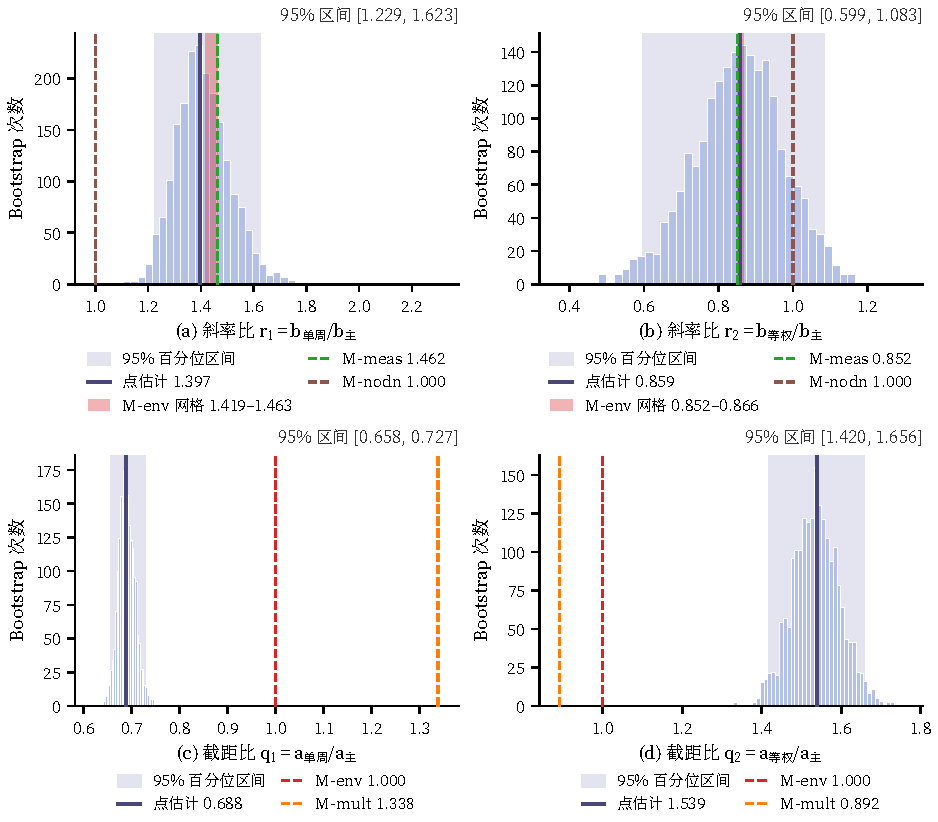
\includegraphics[width=\textwidth]{figures/fig_s1_bootstrap.pdf}
  \caption{滞后权重比值的州聚类重抽分布（$N=1{,}267$ 个州周，$B=2000$，每次重估 $\overline{R}$）。(A) 斜率比 $r_1=b_{\text{单周}}/b_{\text{主}}$；(B) 斜率比 $r_2=b_{\text{等权}}/b_{\text{主}}$；(C) 截距比 $q_1=a_{\text{单周}}/a_{\text{主}}$；(D) 截距比 $q_2=a_{\text{等权}}/a_{\text{主}}$。竖线为点估计，灰带为 95\% 百分位区间，短竖线为各机制的预测（表~\ref{tab:ratios}）。斜率比区间同时容纳平稳环境模型与纯测量误差模型，只排除分母不含计数噪声的模型（仅 $r_1$）；截距比区间排除平稳模型的预测，但与增长期 $\phi=0$ 的日分辨率更新过程及增长期乘性报告噪声的范围相交。}
  \label{fig:s-boot}
\end{figure}

\begin{figure}[!tbp]
  \centering
  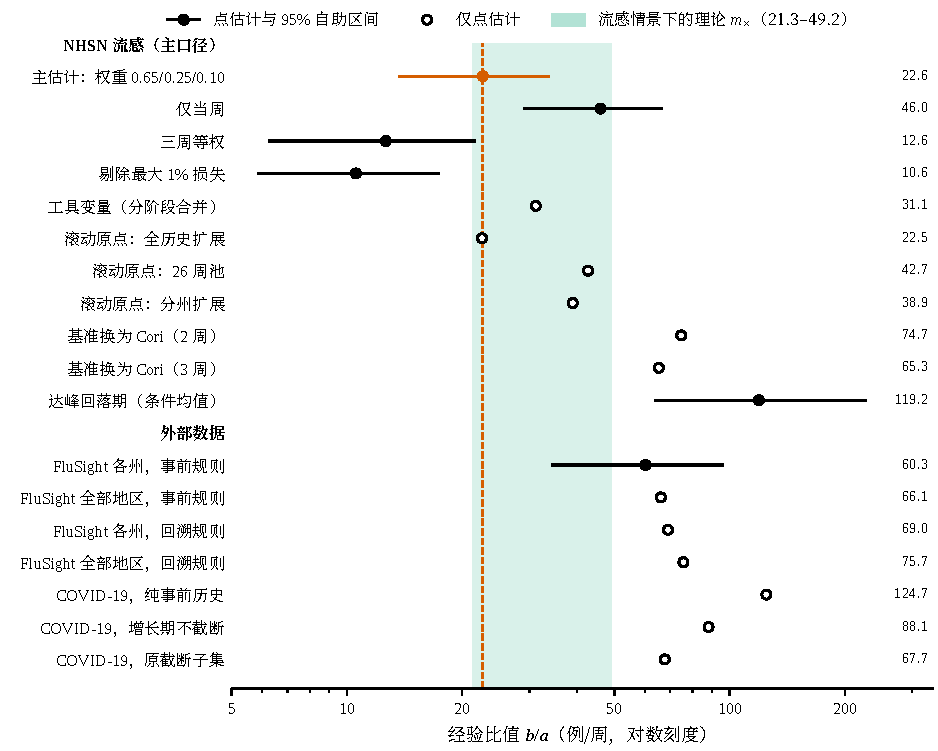
\includegraphics[width=0.96\textwidth]{figures/fig_s2_forest.pdf}
  \caption{各规格下的经验比值 $b/a$（例/周，对数刻度）。横线为原分析按州聚类重抽的 95\% 区间，只有部分规格提供；主估计行 $B=1{,}500$，故与正文 2{,}000 次重抽的 13.5--34.9 略有差别。阴影为流感情景下的理论 $\mx$ 区间 21.3--49.2，竖直虚线为主估计 22.6，右侧列出点估计。上部为 NHSN 流感数据的不同规格，下部为外部数据。}
  \label{fig:s-forest}
\end{figure}

\begin{figure}[!tbp]
  \centering
  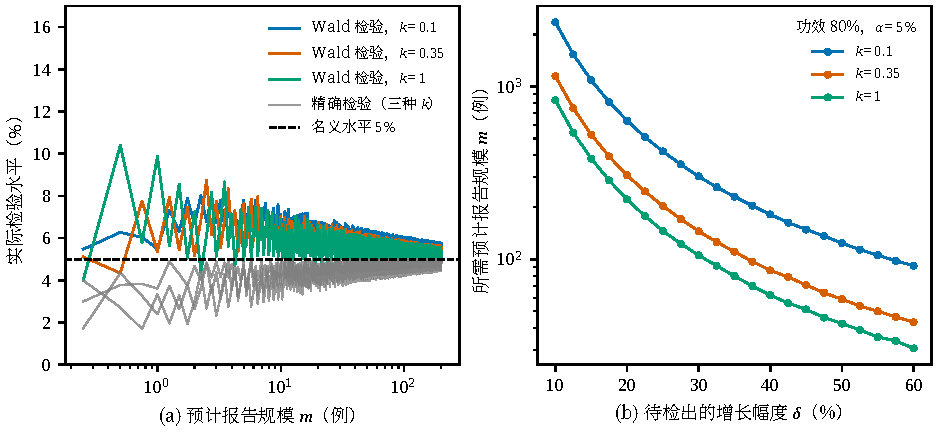
\includegraphics[width=\textwidth]{figures/fig_s3_growth.pdf}
  \caption{增长检验的实际水平与所需规模，$\rho=0.25$，名义水平 5\%，全部由负二项分布函数精确计算，无模拟误差。(A) Wald 检验（按 $k$ 着色）与精确检验（灰色）的实际水平随预计报告规模 $m$ 的变化。(B) 达到并保持 80\% 功效所需的预计报告规模与待检出增长幅度 $\delta$ 的关系。}
  \label{fig:s-growth}
\end{figure}

% Generated by qa/r4_make_supp_tables.py; the tables themselves live in tables/.
\begin{table}[!tbp]
  \centering
  \caption{三种均值形状的比较，主规格流行初期样本（$N=1{,}267$）。各模型用 Gamma 准似然拟合。交叉验证为留一州，基准 $\overline{R}$ 只用训练州估计；差值为相对 M1 的逐州偏差差之和，括号内为州间标准误。}
  \label{tab:shape}
  \small
  \begin{tabular}{@{}llrrrc@{}}
    \toprule
    模型 & 参数估计 & AIC & 交叉验证偏差 & 相对 M1 之差 & 偏向 M1 的州数 \\
    \midrule
    M0：$L=b/D$ & $b=21.7$ & $-1971.2$ & 5407.1 & 1949.9（243.1） & 48/51 \\
    M1：$L=a+b/D$ & $a=0.0991,\ b=2.243$ & $-2718.8$ & 3457.2 & -- & -- \\
    M2：$L=cD^{-p}$ & $c=0.512$，$p=0.273$ & $-2692.6$ & 3514.0 & 56.8（27.2） & 28/51 \\
    \bottomrule
  \end{tabular}
\end{table}

\begin{table}[!tbp]
  \centering
  \caption{滞后权重比值的实证区间与各误差机制的预测（NHSN 流感流行初期，$N=1{,}267$ 个州周）。$r_1$、$r_2$ 为只用当周、三周等权两种权重相对主规格的斜率比，$q_1$、$q_2$ 为对应的截距比，$a$ 为主规格截距。实证区间为按州聚类 $B=2000$ 次重抽的 95\% 百分位区间，每次重抽都重估 $\overline{R}$。平稳环境模型（M-env）的增长期预测有两种，一种是每周一代的更新仿真（$\phi=0$，9 个情景格子，每格 400 次），另一种是 $\phi=0$ 的日分辨率更新过程。后者取流感世代间隔，环境变异系数平方 CV$^2$ 4 档、世代间隔 3 档、增长率 3 档；不含入院延迟时 36 格，加入无、短、长三档入院延迟后共 108 格，每格 300 次。乘性报告噪声模型（M-mult）的平稳行取报告冲击自相关 $\psi$ 遍历 $[0,1)$ 的解析范围（命题~\ref{prop:report-noise}(vi)）。其增长期行取 $v_R=0$ 与对数一阶自回归报告冲击，$\psi\in\{0,0.3,0.6,0.9\}$、$\tau\in\{0.15,0.3\}$、入院延迟 2 档、增长率 3 档，共 48 格，每格 300 次。其余三类为不含环境方差的二项报告模型（M-bin0）、纯测量误差模型（M-meas）与分母不含计数噪声的模型（M-nodn）。区间型预测为各格模拟平均的最小值至最大值。“--”表示该仿真未计算斜率比，“无截距”表示该机制预测 $a=0$、比值无定义。粗体为与实证区间不相交的预测。}
  \label{tab:ratios}
  \footnotesize
  \setlength{\tabcolsep}{4pt}
  \begin{tabular}{@{}lccccc@{}}
    \toprule
    机制 & $r_1$ & $r_2$ & $q_1$ & $q_2$ & $a$ \\
    \midrule
    实证 & 1.397 & 0.859 & 0.688 & 1.539 & 0.0991 \\
    \quad 95\% 百分位区间 & 1.229--1.623 & 0.599--1.083 & 0.658--0.727 & 1.420--1.656 & 0.0837--0.1165 \\
    \midrule
    M-env，平稳 & 1.419--1.463 & 0.852--0.866 & \textbf{1} & \textbf{1} & $>0$ \\
    M-env，增长期，每周一代 & 1.450--1.630 & 0.693--0.763 & \textbf{0.857--0.937} & \textbf{1.226--1.333} & $>0$ \\
    M-env，增长期，日更新无延迟 & -- & -- & \textbf{0.746--0.887} & 1.319--1.484 & $>0$ \\
    M-env，增长期，日更新全部 & -- & -- & 0.601--0.887 & 1.187--1.568 & $>0$ \\
    M-mult，平稳 & 1.462 & 0.852 & \textbf{0.883--1.338} & \textbf{0.892--1.374} & $>0$ \\
    M-mult，增长期 & -- & -- & 0.686--1.224 & 0.865--1.497 & $>0$ \\
    M-bin0 & 1.432 & 0.862 & 无截距 & 无截距 & \textbf{0} \\
    M-meas & 1.462 & 0.852 & 无截距 & 无截距 & \textbf{0} \\
    M-nodn & \textbf{1.000} & 1.000 & \textbf{1} & \textbf{1} & $>0$ \\
    \bottomrule
  \end{tabular}
\end{table}

% Generated by qa/r4_make_supp_tables.py; do not edit by hand.
\begin{table}[!htbp]
  \centering
  \caption{可观测报告贡献 $\Delta a$ 的等价检验（7 个病原与窗口组合，按州聚类 $B=2000$ 次重抽，90\% BCa 区间）。等价界为各组合截距 $a$ 的 5\%；BCa 判定以 90\% 区间落在 $\pm$ 等价界之内为等价，正态判定用重抽标准误的双单侧检验，水平 0.05。$N$ 为州周数，超出量为 $a-0.08/\Rbar^2$。}
  \label{tab:s-tost}
  \small
  \setlength{\tabcolsep}{4pt}
  \begin{tabular}{@{}lrrrrcrcc@{}}
    \toprule
    组合 & $N$ & $a$ & 超出量 & $\Delta a$ & 90\% BCa 区间 & 等价界 & BCa 判定等价 & 正态判定等价 \\
    \midrule
    流感，日历窗口 & 1{,}267 & 0.099 & 0.070 & $-$0.0004 & $-$0.0012--0.0005 & 0.0050 & 是 & 是 \\
    流感，增长期窗口 & 2{,}506 & 0.102 & 0.070 & $-$0.0011 & $-$0.0037--0.0021 & 0.0051 & 是 & 是 \\
    流感，2025--2026 季 & 663 & 0.177 & 0.145 & 0.0039 & 0.0020--0.0060 & 0.0088 & 是 & 是 \\
    COVID-19，日历窗口 & 1{,}479 & 0.037 & $-$0.031 & 0.0001 & $-$0.0004--0.0009 & 0.0018 & 是 & 否 \\
    COVID-19，增长期窗口 & 2{,}774 & 0.023 & $-$0.030 & $-$0.0000 & $-$0.0064--0.0055 & 0.0012 & 否 & 否 \\
    RSV，2024--2025 季 & 494 & 0.080 & 0.037 & 0.0010 & $-$0.0006--0.0023 & 0.0040 & 是 & 否 \\
    RSV，增长期窗口 & 1{,}011 & 0.028 & $-$0.010 & 0.0036 & $-$0.0011--0.0131 & 0.0014 & 否 & 否 \\
    \bottomrule
  \end{tabular}
\end{table}

% Generated by qa/r4_make_supp_tables.py; do not edit by hand.
\begin{table}[!htbp]
  \centering
  \caption{$\Delta a$ 判据在报告率网格上的检验水平与功效（流感日历窗口设定，报告率 $\rho\,h^\kappa u$，35 格，每格 200 次模拟、每次 B=200 次重抽）。$\tau$ 为与填报比例 $h$ 无关的报告离散，$\kappa$ 为报告率对 $h$ 的弹性；$\kappa=0$ 时报告与填报比例无关，判据的拒绝率在全部格中为 0。实证填报比例的中位数为 0.943，$h<1$ 的州周占 0.843。}
  \label{tab:s-tau}
  \small
  \begin{tabular}{@{}lrrrrr@{}}
    \toprule
     & $\kappa=0$ & $\kappa=1$ & $\kappa=3$ & $\kappa=5$ & $\kappa=8$ \\
    \midrule
    \multicolumn{6}{@{}l}{(a) 截距 $a$ 的格点平均} \\
    $\tau=0$ & 0.100 & 0.099 & 0.101 & 0.104 & 0.111 \\
    $\tau=0.05$ & 0.104 & 0.104 & 0.105 & 0.109 & 0.115 \\
    $\tau=0.1$ & 0.118 & 0.118 & 0.118 & 0.121 & 0.127 \\
    $\tau=0.15$ & 0.140 & 0.138 & 0.140 & 0.144 & 0.149 \\
    $\tau=0.2$ & 0.172 & 0.169 & 0.169 & 0.174 & 0.181 \\
    $\tau=0.3$ & 0.257 & 0.255 & 0.251 & 0.255 & 0.265 \\
    $\tau=0.5$ & 0.523 & 0.527 & 0.523 & 0.521 & 0.530 \\
    \addlinespace
    \multicolumn{6}{@{}l}{(b) $\Delta a$ 的格点平均} \\
    $\tau=0$ & $-$0.0016 & $-$0.0004 & 0.0009 & 0.0018 & 0.0028 \\
    $\tau=0.05$ & $-$0.0018 & $-$0.0004 & 0.0008 & 0.0019 & 0.0028 \\
    $\tau=0.1$ & $-$0.0018 & $-$0.0004 & 0.0009 & 0.0019 & 0.0028 \\
    $\tau=0.15$ & $-$0.0019 & $-$0.0006 & 0.0009 & 0.0019 & 0.0029 \\
    $\tau=0.2$ & $-$0.0024 & $-$0.0008 & 0.0009 & 0.0018 & 0.0030 \\
    $\tau=0.3$ & $-$0.0031 & $-$0.0010 & 0.0010 & 0.0017 & 0.0031 \\
    $\tau=0.5$ & $-$0.0060 & $-$0.0032 & 0.0001 & 0.0021 & 0.0033 \\
    \addlinespace
    \multicolumn{6}{@{}l}{(c) $\Delta a$ 的 BCa 区间下端大于 0 的比例} \\
    $\tau=0$ & 0.000 & 0.010 & 0.465 & 0.840 & 0.945 \\
    $\tau=0.05$ & 0.000 & 0.005 & 0.405 & 0.860 & 0.945 \\
    $\tau=0.1$ & 0.000 & 0.025 & 0.415 & 0.820 & 0.920 \\
    $\tau=0.15$ & 0.005 & 0.005 & 0.345 & 0.740 & 0.920 \\
    $\tau=0.2$ & 0.000 & 0.010 & 0.240 & 0.635 & 0.850 \\
    $\tau=0.3$ & 0.000 & 0.020 & 0.220 & 0.465 & 0.735 \\
    $\tau=0.5$ & 0.000 & 0.020 & 0.055 & 0.225 & 0.445 \\
    \addlinespace
    \multicolumn{6}{@{}l}{(d) $\Delta a$ 区间上端与超出量之比的格点中位数} \\
    $\tau=0$ & 0.0000 & 0.0118 & 0.0301 & 0.0460 & 0.0626 \\
    $\tau=0.05$ & 0.0000 & 0.0107 & 0.0280 & 0.0441 & 0.0571 \\
    $\tau=0.1$ & 0.0000 & 0.0092 & 0.0262 & 0.0375 & 0.0506 \\
    $\tau=0.15$ & 0.0000 & 0.0092 & 0.0225 & 0.0334 & 0.0423 \\
    $\tau=0.2$ & 0.0000 & 0.0082 & 0.0185 & 0.0255 & 0.0357 \\
    $\tau=0.3$ & 0.0000 & 0.0065 & 0.0154 & 0.0175 & 0.0251 \\
    $\tau=0.5$ & 0.0000 & 0.0054 & 0.0098 & 0.0126 & 0.0160 \\
    \bottomrule
  \end{tabular}
\end{table}

% Generated by qa/r4_make_supp_tables.py; do not edit by hand.
\begin{table}[!htbp]
  \centering
  \caption{各流行季截距与季随机效应合并（NHSN 流感，按州聚类 $B=2000$ 次重抽的 95\% 百分位区间；合并为 DerSimonian--Laird 估计与 $t_{S-1}$ 区间，季间方差 $\hat v_S$ 的区间为 Q-profile 法）。(a) 各季估计，SE 为州聚类重抽标准误。(b) 合并结果；最后一列为推论~\ref{cor:season} 的相对标准误下界 $\sqrt{2/S}$ 与 $\sqrt{2/(S-1)}$。第 4 季取窗规则与前三季不同，$S=4$ 只作敏感性参照。}
  \label{tab:s-seasons}
  \small
  \begin{tabular}{@{}lrrrr@{}}
    \toprule
    (a) 流行季 & $N$ & $a$ & 95\% 区间 & SE \\
    \midrule
    2022--23 季（日历窗口） & 338 & 0.071 & 0.049--0.094 & 0.0121 \\
    2023--24 季（日历窗口） & 419 & 0.028 & 0.017--0.041 & 0.0077 \\
    2024--25 季（日历窗口） & 510 & 0.135 & 0.111--0.166 & 0.0139 \\
    2025--26 季（增长期规则，样本外） & 663 & 0.177 & 0.141--0.212 & 0.0186 \\
    \bottomrule
  \end{tabular}

  \medskip
  \begin{tabular}{@{}lrrrrrrr@{}}
    \toprule
    (b) 合并 & $a_{\mathrm{RE}}$ & 95\% $t$ 区间 & $\hat v_S$ & Q-profile 区间 & $Q$ & $I^2$ & 下界 \\
    \midrule
    $S=3$ & 0.077 & $-$0.056--0.211 & 0.0028 & 0.0007--0.1155 & 47.4 & 0.958 & 0.82 / 1.00 \\
    $S=4$ & 0.101 & $-$0.002--0.205 & 0.0041 & 0.0012--0.0609 & 85.0 & 0.965 & 0.71 / 0.82 \\
    \bottomrule
  \end{tabular}
\end{table}

% Generated by qa/r4_make_supp_tables.py; do not edit by hand.
\begin{table}[!htbp]
  \centering
  \caption{世代块长度为 7 天与 4 天时的模拟截距与截距比（流感日历窗口设定，世代间隔中档，环境变异系数平方 $\CV^2=0.0287$，60 格中的 20 格，每格 300 次模拟的平均）。$\phi$ 为周尺度的环境自相关，4 天块取 $\phi^{4/7}$；“长”为长入院延迟。星号标出同时落入实证 $a$ 的 95\% 百分位区间与 $q_1$、$q_2$ 的 95\% BCa 区间的格。全部 30 对格中，两种块长之差的最大绝对值为 $a$ 0.088、$q_1$ 0.029、$q_2$ 0.049。实证值为 $a=0.099$、$q_1=0.688$、$q_2=1.539$、$b/a=22.6$。}
  \label{tab:s-twogen}
  \small
  \begin{tabular}{@{}llrrrrrrrr@{}}
    \toprule
    $\phi$ & 延迟 & $a$（7 天） & $a$（4 天） & $q_1$（7 天） & $q_1$（4 天） & $q_2$（7 天） & $q_2$（4 天） & $b/a$（7 天） & $b/a$（4 天） \\
    \midrule
    0 & 无 & 0.100 & 0.056 & 0.824 & 0.816 & 1.381 & 1.398 & 14.2 & 25.5 \\
    0 & 长 & 0.073 & 0.044 & 0.722 & 0.727 & 1.528 & 1.518 & 18.6 & 30.7 \\
    0.3 & 无 & 0.126 & 0.109$^{*}$ & 0.735 & 0.712 & 1.512 & 1.546 & 10.6 & 12.2 \\
    0.3 & 长 & 0.102$^{*}$ & 0.094$^{*}$ & 0.680 & 0.677 & 1.603 & 1.607 & 12.7 & 14.0 \\
    0.5 & 无 & 0.143 & 0.132 & 0.693 & 0.675 & 1.584 & 1.611 & 8.2 & 9.3 \\
    0.5 & 长 & 0.123 & 0.121 & 0.658 & 0.657 & 1.645 & 1.639 & 9.7 & 9.7 \\
    0.7 & 无 & 0.157 & 0.150 & 0.665 & 0.655 & 1.645 & 1.657 & 6.0 & 6.7 \\
    0.7 & 长 & 0.144 & 0.142 & 0.646 & 0.645 & 1.679 & 1.679 & 6.8 & 7.0 \\
    0.9 & 无 & 0.149 & 0.148 & 0.650 & 0.648 & 1.705 & 1.709 & 5.2 & 5.1 \\
    0.9 & 长 & 0.147 & 0.147 & 0.649 & 0.646 & 1.712 & 1.715 & 5.0 & 5.0 \\
    \bottomrule
  \end{tabular}
\end{table}

% Generated by qa/r4_make_supp_tables.py; do not edit by hand.
\begin{table}[!htbp]
  \centering
  \caption{非 NHSN 数据的截距比（2022--2025 年日历窗口，与主分析相同的管线，按辖区或站点聚类 $B=2000$ 次重抽的 95\% 百分位区间）。末列为重抽中同时满足 $q_1<1<q_2$ 的比例。HHS Protect 医院日报与 NHSN 在 3{,}417 个州周上的相关系数为 0.995，相对差的中位数为 0.074，只作数据一致性核对。病例定义与 NHSN 不同，两组结果都不参与分级。}
  \label{tab:s-indep}
  \small
  \begin{tabular}{@{}llrllr@{}}
    \toprule
    数据 & 聚类单元 & $N$ & $q_1$ & $q_2$ & 方向一致比例 \\
    \midrule
    ILINet 门诊流感样病例 & 51 个辖区 & 1{,}479 & 0.687（0.552--0.842） & 1.467（1.406--1.531） & 0.997 \\
    FluSurv-NET 住院率 & 14 个站点 & 364 & 0.686（$-$3.608--3.920） & 1.312（$-$4.382--7.217） & 0.560 \\
    \bottomrule
  \end{tabular}
\end{table}

% Generated by qa/r4_make_supp_tables.py; do not edit by hand.
\begin{table}[!htbp]
  \centering
  \caption{零假设范围的取法与分级（7 个病原与窗口组合，按州聚类 $B=2000$ 次重抽的 95\% BCa 区间）。零假设范围为日分辨率更新过程（108 格）与增长期乘性报告噪声模型（48 格）格点平均的最小值至最大值，每格 300 次模拟。分级列：主为事先写定的取法（全部格）；无延迟只用不含入院延迟的日更新格；每周一代为正文第~\ref{sec:res-inflation}~节每周一代仿真的增长期范围。中位数与均值之比为事后取法，以格点中位数或格点均值之比代替格点平均。“部分”为部分复现，“方向”为方向一致。}
  \label{tab:s-grading}
  \scriptsize
  \setlength{\tabcolsep}{2.5pt}
  \begin{tabular}{@{}lrllllllllll@{}}
    \toprule
    组合 & $N$ & $q_1$ 区间 & $q_2$ 区间 & $q_1$ 零假设范围 & $q_2$ 零假设范围 & 超出量区间 & 主 & 无延迟 & 每周一代 & 中位数 & 均值之比 \\
    \midrule
    流感，日历窗口 & 1{,}267 & 0.656--0.727 & 1.422--1.655 & 0.601--1.224 & 0.865--1.568 & 0.0530--0.0867 & 部分 & 部分 & 复现 & 部分 & 部分 \\
    流感，增长期窗口 & 2{,}506 & 0.487--0.643 & 1.686--2.261 & 0.625--1.242 & 0.863--1.578 & 0.0455--0.0945 & 部分 & 复现 & 复现 & 复现 & 复现 \\
    流感，2025--2026 季 & 663 & 0.575--0.715 & 1.430--1.657 & 0.639--1.240 & 0.864--1.569 & 0.1100--0.1850 & 部分 & 部分 & 复现 & 部分 & 部分 \\
    COVID-19，日历窗口 & 1{,}479 & 0.652--0.799 & 1.393--1.676 & 0.558--1.279 & 0.893--1.763 & $-$0.0415--$-$0.0112 & 方向 & 方向 & 部分 & 方向 & 方向 \\
    COVID-19，增长期窗口 & 2{,}774 & 0.688--0.988 & 1.174--1.642 & 0.610--1.272 & 0.885--1.653 & $-$0.0400--$-$0.0154 & 方向 & 方向 & 方向 & 方向 & 方向 \\
    RSV，2024--2025 季 & 494 & 0.618--0.774 & 1.381--1.799 & 0.210--3.679 & $-$1.888--1.609 & 0.0245--0.0509 & 部分 & 复现 & 复现 & 部分 & 部分 \\
    RSV，增长期窗口 & 1{,}011 & 0.520--0.803 & 1.281--2.061 & 0.539--1.266 & 0.861--1.547 & $-$0.0187--0.0057 & 方向 & 方向 & 方向 & 方向 & 方向 \\
    \midrule
    计数（复现/部分/方向） & & & & & & & 0/4/3 & 2/2/3 & 4/1/2 & 1/3/3 & 1/3/3 \\
    \bottomrule
  \end{tabular}
\end{table}


\FloatBarrier

\section{复现包}
\label{sec:s-repro}

分析代码、数据快照的校验值与结果文件公开于 \url{https://github.com/wangchi2068/case-count-bottleneck}，投稿时另在 Zenodo 存档并给出 DOI。

\paragraph{结构} \nolinkurl{code/} 为全部分析脚本，\nolinkurl{analysis/} 为结果文件（\nolinkurl{reanalysis_results.json}、\nolinkurl{r3_results.json}、\nolinkurl{r4_results.json}）、事先写定的分析方案与数字地图，\nolinkurl{data/} 为派生面板与外部数据，\nolinkurl{logs/} 为运行日志。论文中每个数字对应的结果键列在 \nolinkurl{analysis/reproduction_map.md}，共抽取 1,638 个数字，其中 1,550 个映射到结果键，其余为年份、参数设定与理论部分的闭式计算。

\paragraph{环境} Python 3.11.2、numpy 2.4.6、scipy 1.17.1、pandas 3.0.6、matplotlib 3.11.2，不调用外部接口（独立数据脚本首次运行时从公开接口下载，文件已存在时不再访问网络）。参考硬件为 4 核 CPU、8 GiB 内存，无 GPU。

\paragraph{数据} 主数据为 NHSN 州级每周住院数据（Weekly Hospital Respiratory Data Metrics by Jurisdiction）的论文快照，sha256 为 \texttt{e48c2ea9\dots c20c330}。该数据集持续回填，逐值复现须使用快照；ILINet、FluSurv-NET 与 HHS Protect 文件的来源与校验值见代码目录的说明文件。

\paragraph{种子} 主种子为 20261017。首轮州聚类重抽用主种子；跨病原重抽为 20261022；日分辨率更新过程零假设为 20261058，乘性报告噪声增长期模型为 20261059，报告率网格为 20261060，一周两代为 20261061，独立数据为 20261062。每格的随机数流只由种子与格号决定，与进程数和完成顺序无关。

\paragraph{运行顺序} \nolinkurl{bash run_all.sh} 按依赖顺序执行 21 条命令，分 base、r3、r4、map 四个阶段，各命令的产出键与参考耗时列在说明文件中；最耗时的是零假设仿真，4 进程约 45--60 分钟。

\paragraph{复现核对} 把 \nolinkurl{code/} 复制到空目录后重跑表~\ref{tab:ratios} 与图~\ref{fig:pathogens} 所需的全部步骤，与原结果逐值比较（容差 $10^{-9}$），24,815 个数值无一不一致，表~\ref{tab:ratios} 的 LaTeX 源逐字相同。

\end{document}
